% Chapter 6

\begin{savequote}[\quotewidth] I'm really into coconut oil for everything. I cook it,
eat it, put it in my hair, and use it as body lotion. I put it on my face, too -
day cream, night cream, whatever. I love the smell. It reminds me of the beach.
I'm not particular on what brand as long as it's organic.

\qauthor{Actress Juliette Lewis, observing the oxidative stability of coconut oil.}
\end{savequote}

\chapter{Investigating biodiesel feedstock using SFC×GC} % Main chapter title

\label{Chapter6} % For referencing this chapter elsewhere, use \ref{Chapter6}

\section{Introduction}


Biodiesel consists mostly of a mixture of methyl esters of fatty acids obtained
from plant oils. To comply with the relevant technical standard, \std{SANS 1935},
\autocite{SANS1935} (see Chapter \ref{Chapter3}), it must consist of a mass
fraction of \SI{96.5}{\percent} or more of fatty acid methyl esters (FAME), but
not more than \SI{12}{\percent} linolenic acid methyl ester, and not more than
\SI{1}{\percent} of FAMEs with more than \num{4} double bonds. The prescribed
methods for determining the quantities of these compounds are chromatographic,
but the method for  determining the \emph{total amount} of FAMEs differs
completely from the method for determining the amount of \emph{unsaturated}
FAMEs. Both these methods generate complex chromatograms that need highly
skilled and experienced chromatographers to interpret. There is no doubt that
the use of artificial intelligence and other technological innovations for
interpreting chromatograms will grow, but the paradox of
automation\footnote{Automation helps you least when you need it most
\autocite{Strauch2018, Bainbridge1983}.} predicts that as biodiesel production
grows, feedstocks proliferate, and complexity increase, the analytical chemist
will need better tools, methods, and instruments to understand the problems that
arise when automation fails. Comprehensively coupled chromatography offers a way
to better exploit chemistry for improved analytical separations, adding another
tool to the analytical chemist's toolbox. It does this in three ways: the first is
by increasing the peak capacity of the system, the second is by improved
sensitivity, and the third is by generating patterns in the data.

\section{SFC of FAMEs}

The power of comprehensive chromatography is unlocked by orthogonality.
Orthogonality is the difference in separation mechanism between the two
dimensions \autocite{Marriott2012}. When FAMES are chromatographically separated
by SFC using neat carbon dioxide as a mobile phase and unmodified silica as a
stationary phase, the separation is according to the number of double bonds,
independent of chain length \autocite{Robertson1991, Smith1994, Smith2001}. This
stands in strong contrast to the separation of FAMEs by GC, where the major
separation is according to volatility, which can be adjusted --- but not
overridden --- by changing the polarity (or other chemical aspect) of the
stationary phase (See Figure \ref{fig:RestekFAMEsGC}).

\begin{figure}
\centering
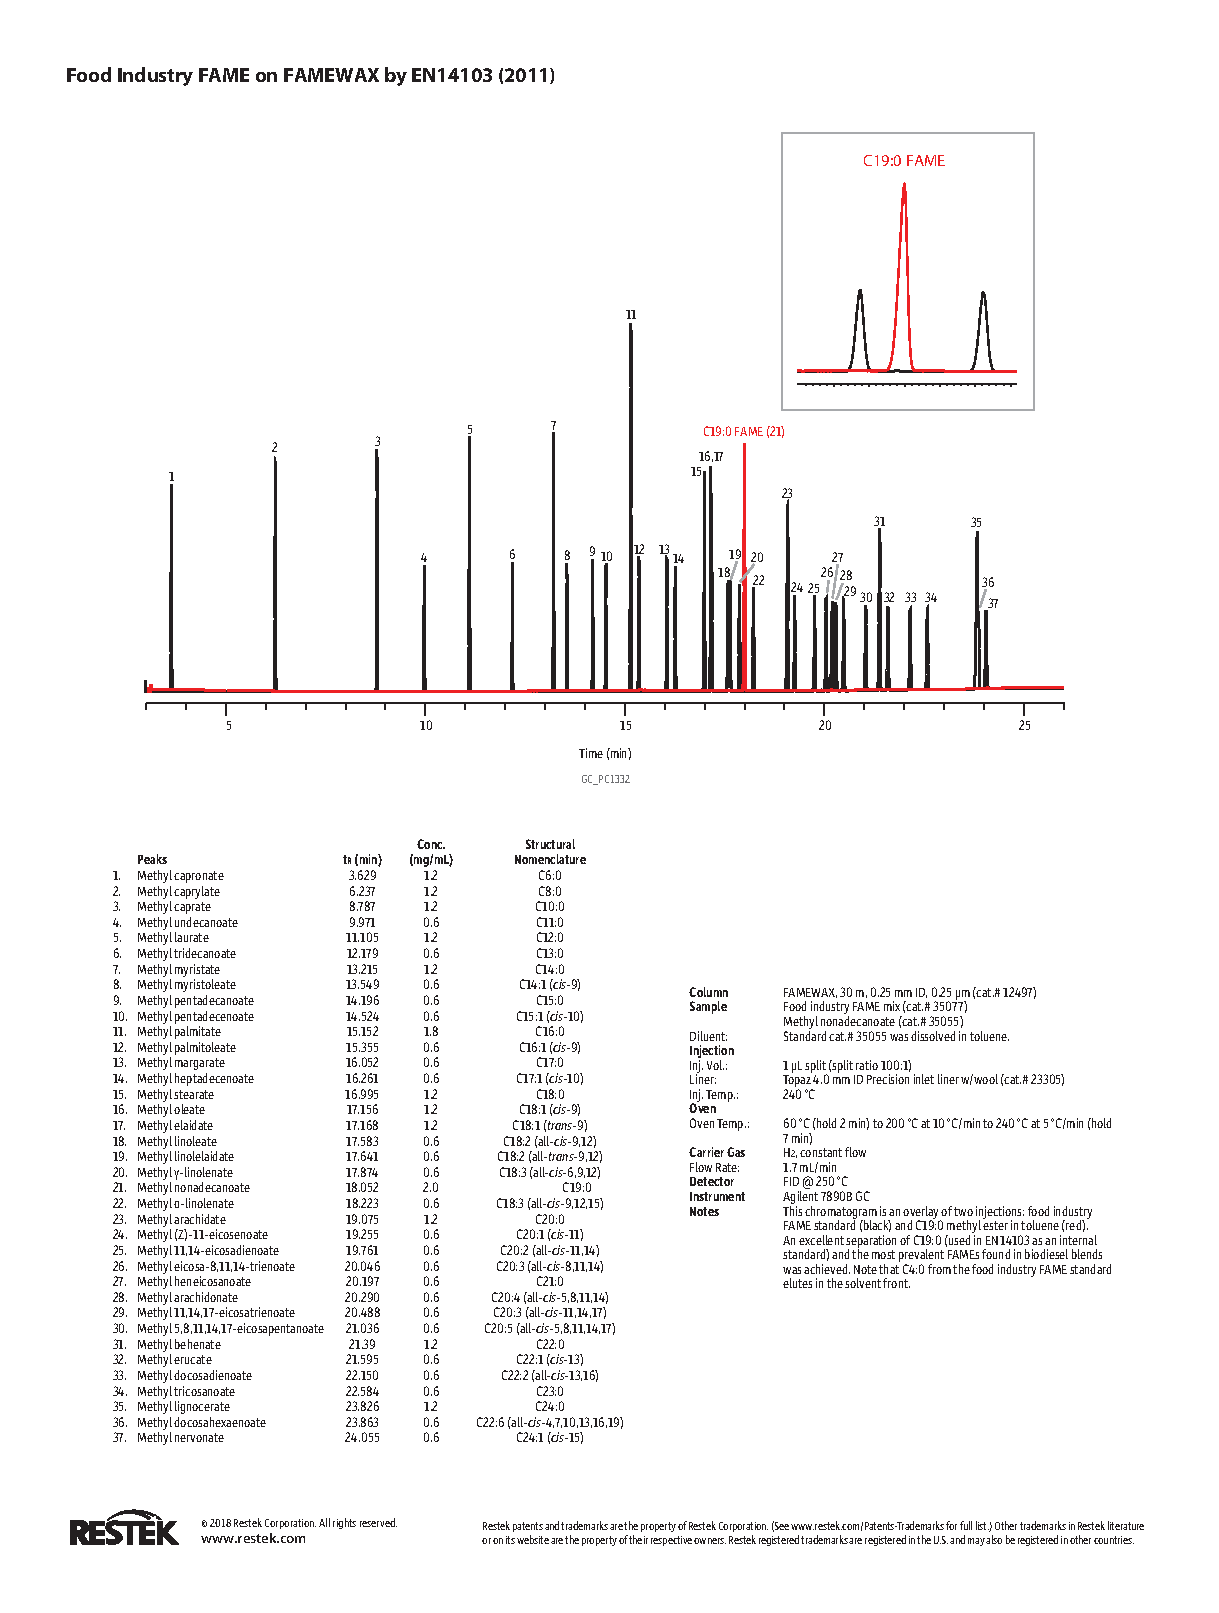
\includegraphics[width=\textwidth]{Figures/GC_PC1332.pdf}
\decoRule

\caption[Separation of FAMEs by GC]{This figure shows that when separating FAMEs
by GC, using a specialized column, separation is primarily by fatty acid chain
length, and secondarily by number of double bonds. Reproduced with permission of
Restek Corporation.}

\label{fig:RestekFAMEsGC}
\end{figure}

Silver ions are often used in stationary phases to separate unsaturated
compounds, and this includes stationary phases for SFC \autocite{Sandra2002,
Potgieter2013}. The retention mechanism is quite complex
\autocite{Nikolova-Damyanova2019}, but it offers a powerful technique for the
elucidation of lipid structures, as reviewed as early as 1966
\autocite{Morris1966}. Nevertheless, in this chapter the use of stationary
phases modified with silver ions was neither necessary nor attempted.

%As discussed in Section \ref{sec:Rancimat}, fatty acids are not stable at high
%temperatures. This means that they might degrade during chromatographic
%separation at high temperature, especially if the run times are long. Because
%SFC operates at low temperatures, the unstable compounds are less likely to
%degrade.

The utterly different retention behaviours of FAMEs on silica with a carbon
dioxide mobile phase and on GC offers high orthogonality, which promises to make
comprehensive coupling worthwhile.

\section[Coaxial heater performance.]{Performance of the coaxial heater.}

Practical SFC×GC depends on reliably repeating fast temperature programs on a
capillary gas chromatography column. The effect of these conditions on the
column will be discussed in the following sections.

\subsection{Column lifetime}

As discussed in Section \ref{sec:ChromDet}, FAMEs can be separated by gas
chromatography using relatively non-polar columns with high-temperature
programs. For this purpose column manufacturers supply special 'high
temperature' columns, which address two aspects of column lifetime: mechanical
degradation and stationary phase degradation. The SFC×GC chromatograph did not
use such columns, and the following discussion explains why their use could be
avoided.

\subsubsection{Mechanical degradation}
Fused silica has a high \keyword{tensile strength}, but also a low
\keyword{fracture toughness}. This means that it is strong enough to resist the
forces involved in its use as a column, but very liable to fracture if it gets
damaged. Very small flaws, less than a micron in depth, will cause fused silica
(or any other glass) to fracture under loads far under what would be expected
from its tensile strength. Such flaws can be caused by mechanical scratches or
reaction with atmospheric water. To prevent this the outside of the fused silica
capillary is coated with a protective layer of \keyword{polyimide resin}. The
strength of the a capillary column therefore depends on the integrity of the
polyimide coating. Like all resins and polymers, the polyimide coating degrades
faster at higher temperatures, so the longer the column spends at high
temperature the sooner the polyimide will degrade to the point where it fails to
protect the fused silica, and the shorter the overall mechanical lifetime of the
column will be.

Traditionally, chromatographers are advised to use temperature programs that
minimize the time spent at high temperature, which will contribute to longer
column lifetimes. The usual way to do it is to use a temperature program with
a maximum temperature no higher than necessary, but the same cumulative time at
high temperature can be obtained by using higher temperatures but for shorter
periods. Fast temperature programs expose the columns to high temperatures for
only very brief periods.

(Column mechanical lifetime can also be improved by using metal capillaries.
Metals are not afflicted by brittle fracture the way fused silica is, but they
don't offer the chemical inertness of fused silica. To exploit the fracture
toughness of metal, technologies have been developed to deactivate metal surfaces
\autocite{Rohwer1986, Smith2002}, which makes metal columns a modern
possibility. Column manufacturers offer metal columns specifically designed for
biodiesel analysis.)

Another durability benefit of the stainless steel coaxial heater is that the
outer surface of the capillary column is protected from mechanical damage by its
encasement in the stainless steel tube of the coaxial heater. During development
of the coaxial heater there were occasions where the column was accidentally
overheated by poorly-controlled resistive heating. Even though the polyimide
coating had been completely charred away and the capillary was left fragile, the
column was intact and still provided separations.

Using carbon dioxide as a between-program coolant also protects the polyimide
coating from oxidative damage by purging the column environment of oxygen.

\subsubsection{Stationary phase degradation}

The stationary phases inside the GC columns face degradation similar to that of
the polyimide. Column manufacturers minimize sta\-tion\-ary phase degradation by
using improved technologies like cross-linked resins, or polymers with backbones
resistant to certain degradation mechanisms \autocite{Day2003}.
Fast temperature programs help extend stationary phase lifetime by minimizing
the cumulative time the column spends at high temperature.

\subsubsection{Column bleed}
Short columns and fast temperature programs have another beneficial side effect:
reduced \keyword{column bleed}. Any resin- or polymer-based stationary phase
degrades over time, and this degradation is faster at higher temperatures
\autocite[p. 66]{Mcnair2019}. It is observed as a rise in baseline during the
high temperature part of a temperature program. Various stationary phase
technologies can be employed to reduce column bleed, but because the amount of
column bleed depends on the amount of stationary phase it is clear that a
\SI{1}{\metre} column will have \num{1/30}th of the column bleed of a
\SI{30}{\metre} column with the same stationary phase. Despite using temperature
programs that went up to the temperature limit recommended by the column
manufacturer, column bleed was not a significant feature in the obtained
chromatograms.

\subsection{Thermal shock}
An aspect of fast temperature programming with such a temperature range as used
in this study (\SIrange{-30}{400}{\celsius}) is \keyword{thermal shock}. Thermal
shock occurs when an object is subjected to a rapid change in temperature. Under
such non-equilibrium conditions different parts of the object will have
different temperatures. The material that the object is made of has a certain
\keyword{coefficient of thermal expansion}, which means that the relative sizes
of the parts of the object at different temperatures will change at different
rates. This will cause stress between the parts, and if the stress exceeds the
strength of the material, the material will fracture. Fused silica has a low
coefficient of expansion\footnote{\SI{0.55e-6}{\per\kelvin}, compared to the
\SI{9.0e-6}{\per\kelvin} of soda lime glass or the \SI{4.0e-6}{\per\kelvin} of
borosilicate glass}, and therefore experiences low thermal shock. The amount of
material in a capillary is also relatively small, which keeps temperature
gradients small and therefore stresses low. No column failures that could be
ascribed to thermal shock were observed.

\subsection{Thermal fatigue}

Another cause of material failure due to temperature is \keyword{thermal
fatigue}. ``Thermal fatigue (TF) is the gradual deterioration and eventual
cracking of a material by alternate heating and cooling during which free
thermal expansion is partially or completely constrained'' \autocite{Rao2001}.
The expansion of the portion of the fused silica column subjected to alternate
heating and cooling is not constrained, and the part of the fused silica column
that is constrained (in the sealing ferrules) is not subjected to alternate
heating and cooling (it is held at constant temperature in the heated T-piece
block), therefore thermal fatigue is not expected. No explicit test for thermal
fatigue was performed, but no column failure that could be attributed to thermal
fatigue was observed.

\subsection{Corrosion}
One failure of the coaxial heater could be attributed to corrosion. The joint
between the coaxial heater and the heated T-piece block is brazed, and there was
a failure of the thin-walled stainless steel tube near that joint in the portion
heated during the brazing operation. Visual inspection seemed to indicate
thinning caused by corrosion. An acid flux was used during the brazing, which
might have contributed to the corrosion, especially in the presence of water
condensed from the atmosphere during the cooling of the column.

\subsection{GC retention time precision}

During the development of the resistive heater it was shown that the measured
temperature ramps are highly repeatable. But the retention times of  compounds
being separated by GC are highly sensitive to temperature, so it was necessary
to obtain a measure of the retention time repeatability.

To estimate the retention time variance, two alkanes (dodecane and hexadecane)
were added to the SFC mobile phase at a concentration of about
\SI{0.6}{\percent}. These compounds are not retained on the silica at all, and
are therefore present in all the GC runs at the same concentration and all the
peaks should be identical. Variance in retention time, peak area, and peak
height therefore indicate the repeatability of the fast GC system. Variability
of retention time is summarized in Table \ref{tab:RetentionTimeVariance}.

\begin{table}[ptbh]

	\caption{\label{tab:RetentionTimeVariance}A summary of retention time repeatability of alkanes
separated on the fast temperature programmed chromatograph.}
	\centering
	\begin{tabular}{lllll}
	\toprule
	\tabhead{Compound} & \tabhead{n} & \tabhead{t\textsubscript{r} (s)} & \tabhead{S.D. of t\textsubscript{r} (s)}	& \tabhead{R.S.D. of t\textsubscript{r} (\%)} \\
	\midrule
	Dodecane 			& 73 		& 5.07 								& 0.023 									& 0.46\\
	Hexadecane			& 73 		& 6.58 								& 0.052 									& 0.78\\
	\bottomrule
\end{tabular}

\end{table}

The peak widths were about \SI{500}{\milli\second}, so the
\SI{20}{\milli\second} standard deviation for hexadecane means that the
variation in retention time is only about \SI{10}{\percent} of the peak width.
The relative standard deviations (RSD) of retention times were similar to those
obtained in GC×GC \autocite{Shellie2002}, and much smaller than those of our
original ``proof of concept'' instrument , for which standard deviations of
\SI{0.080}{\second} and \SI{0.087}{\second} were reported for dodecane and
hexadecane respectively \autocite{Venter2003, Venter2004}.

\subsection{Coolant consumption}

In Section \ref{sec:ColdColumn} it was mentioned that the first SFC×GC
instrument consumed many kilograms of carbon dioxide coolant for each run. With
coaxial cooling, if a typical SFC×GC run consists of \num{200} GC runs which
each requires \SI{7}{\second} of coolant flow at a rate of
\SI{30}{\gram\per\minute}, then \SI{700}{\gram} of carbon dioxide coolant would
be consumed per run, an order-of-magnitude improvement.

\section[Study of biodiesel feedstock by SFC×GC]{Study of potential biodiesel feedstock by SFC×GC}

Biodiesel can be produced from any combination of a variety of vegetable
oils\footnote{At this time \std{SANS 1935} excludes animal fats, but they might be
included in future. All of the following discussion also applies to animal
fats.}. Indeed, to ensure conformance to standards it might be necessary to
produce biodiesel from blends or combinations of oils. But as an introduction it
is instructive to start by analysing the FAMEs obtained from neat oils.

\subsection{Samples}

Various samples of edible oil were obtained from supermarkets. (See Table
\ref{tab:OilSamples})

\begin{table}[hptb]
	\caption{Oils used for FAME analysis}
	\label{tab:OilSamples}
	\centering
	\begin{tabular}{l l l}
	\toprule
	\tabhead{Oil} & \tabhead{Brand} & \tabhead{Species} 			\\
	\midrule
	Canola			& Spar			& \textit{Brassica napus}		\\
	Sunflower oil	& Pick n Pay 	& \textit{Helianthus annuus}	\\
	Coconut oil  	& Lemcke 		& \textit{Cocos nucifera}		\\
	Flax seed oil 	& Lemcke 		& \textit{Linum usitatissimum}	\\
	Salmon oil		& Dis-Chem Gold & Family \textit{Salmonidae}		\\
	\bottomrule\\
	\end{tabular}
\end{table}

\subsection{Sample preparation}

Fatty acids in oils might be either free or bound to glycerol. To quantitatively
convert them to FAMEs therefore requires that the bound fatty acid be
transesterified, and the free fatty acids esterified. Both transesterification
and esterification can be achieved by acid catalyst, but this reaction is quite
slow. Basic catalysts can rapidly transesterify acyl glycerols, but will not
esterify free fatty acids.

The method used involved first treating the oil sample with sodium hydroxide
dissolved in dry methanol. The methanol acts as a solvent but also provides an
excess of methanol so that the transesterification reaction is driven to
completion. On completion of the reaction an excess of acid is added, which
neutralizes the base and esterifies any free fatty acids. Then an organic
solvent and water are added, which provides two phases: the non-polar FAMEs
dissolve in the organic layer, and the polar glycerol and salts dissolve in the
water layer.

\subsubsection{Method}

This method is based on an official method \autocite{AOCS2017}, modified in two
respects. Firstly, the acidic catalyst boron trifluoride is replaced by
sulphuric acid, and secondly, hexane is used instead of heptane.

\begin{enumerate}
  
\item Transfer \num{4} drops of melted sample to a \SI{20}{\milli\litre} glass
stoppered test tube. Add a few boiling stones.

\item Add \SI{2}{\milli\litre} NaOH/methanol solution (0.5N) and boil for
\SI{11}{\min} under reflux.

\item Add \SI{2}{\milli\litre} 10\%
H\textsubscript{2}SO\textsubscript{4}/methanol solution via the condenser and
boil for \SI{2}{\minute}.

\item  Add \SI{2}{\milli\litre} hexane via the condenser and boil for
\SI{1}{\minute}.

\item Remove the test tube from the heat source and leave to cool.

\item Add \SI{4}{\milli\litre} saturated NaCl solution and mix gently.

\item Allow the phases to separate. Transfer the hexane layer to a vial and use
for injection.

\end{enumerate}

\subsection{SFC}

A \SI{0.5}{\micro\litre} volume of the hexane layer was injected into the neat
carbon dioxide mobile phase as described in Section \ref{sec:SFCInjection}. The
column was five HPLC columns (150 mm $\times$ 4.6 mm, 3 $\mu$m particles)
(Restek, Pinnacle DB Silica) connected in series.

\subsection{Modulation}

The modulation period was \SI{10}{\second}, during which the fractions of the SFC
eluate were transferred to the GC inlet via a linear restrictor. In the hot
(\SI{350}{\celsius}) inlet the fractions evaporated instantly and were swept onto the
cold (\SI{-20}{\celsius}) column where they were trapped in the stationary phase.
\SI{3}{\second} after the collection period ended the vent valve opened for
\SI{1}{\second} to vent excess pressure from the GC inlet.

\subsection{GC}

The fast temperature program ramped the GC column temperature from
\SI{-20}{\celsius} to \SI{350}{\celsius} in \SI{10}{s}
(\SI{2220}{\celsius\per\minute}), maintaining \SI{350}{\celsius} for
\SI{2}{\second}. Then the cooling system activated and cooled the column to
\SI{-20}{\celsius} or below, ready to trap the next SFC fraction. The FID
detector was kept at \SI{350}{\celsius}.

In this way a series of GC chromatograms of SFC fractions were recorded, which
were assembled into a 2D chromatogram. Figure \ref{fig:2DCanola} shows a 2D
chromatogram of a sample of FAMEs prepared from canola oil. This 2D chromatogram
consists of 132 fast GC chromatograms collected in approximately 90 minutes.

\subsection{Results and discussion}

\begin{figure}
\centering
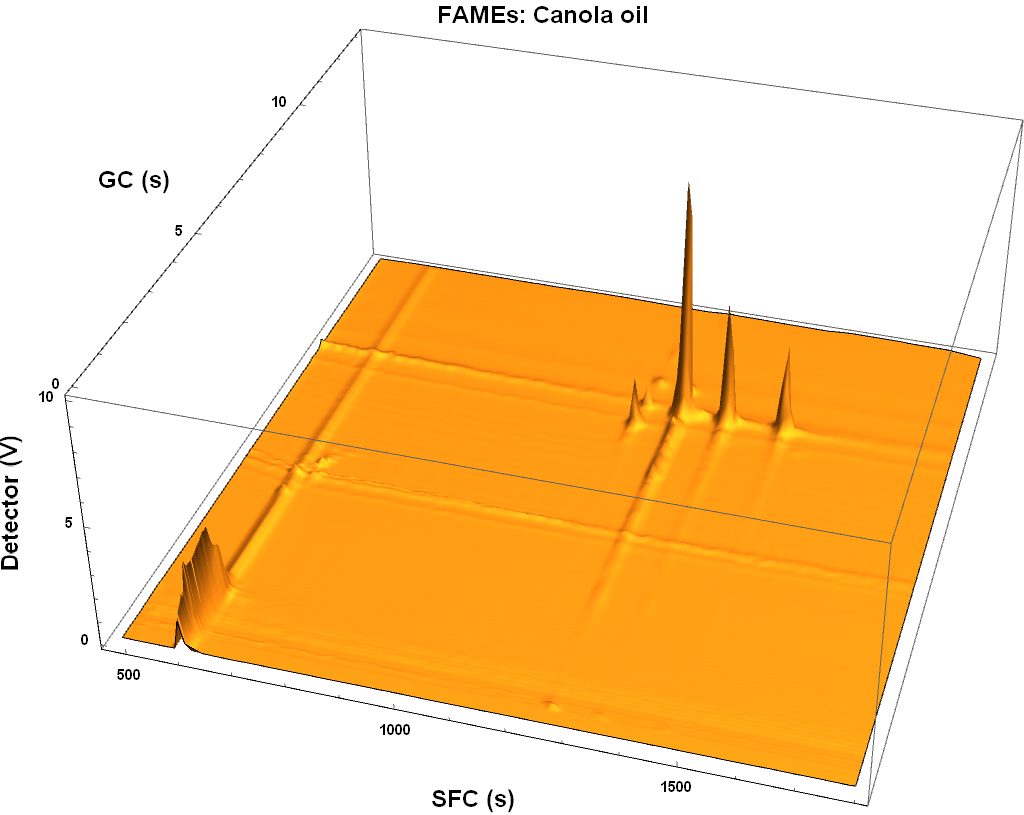
\includegraphics[width=\textwidth]{Figures/Canola.png}
\decoRule

\caption[SFC×GC of canola oil]{A 2D chromatogram of FAMEs derived from
canola oil. It is clear that the oil consists mostly of unsaturated fatty
acids.}

\label{fig:2DCanola}
\end{figure}

The chromatogram shown in Figure \ref{fig:2DCanola} is very simple to interpret.
In the SFC dimension, separation is by number of double bonds.
This means that FAMEs without double bonds elute first in this dimension,
followed by FAMEs with one, two and three double bonds respectively. There is
good resolution between the peaks in the SFC dimension.

The volatility of a FAME depends primarily on the length of the carbon atom
chain, therefore the separation in the GC dimension is by chain length. Because
these FAMEs are of biological origin, we expect their chains to have an even
number of carbon atoms. From the literature we know that oleic acid (C18:1) is
the most common fatty acid in canola oil \autocite{JFAOWHOCAC2019}, and that
therefore the major peak in the chromatogram is a C18 FAME. This allows us to
easily identify the peaks for C16, C18, C20, and C22 in the GC dimension.

The information provided by this chromatogram confirms that canola oil is a
vi\-able bio\-diesel feedstock: The unsaturated compounds have mostly a single
double bond, which should make it oxidatively stable (\label{sec:Rancimat}), and
the quantities of unsaturated FAMEs are low, which means that it will most
likely have suitable cold-flow properties (see Section \ref{sec:CFPP}), because
the naturally occurring \textit{cis} isomers of unsaturated FAMEs have higher
freezing points than their saturated analogues.

\begin{figure}
\centering
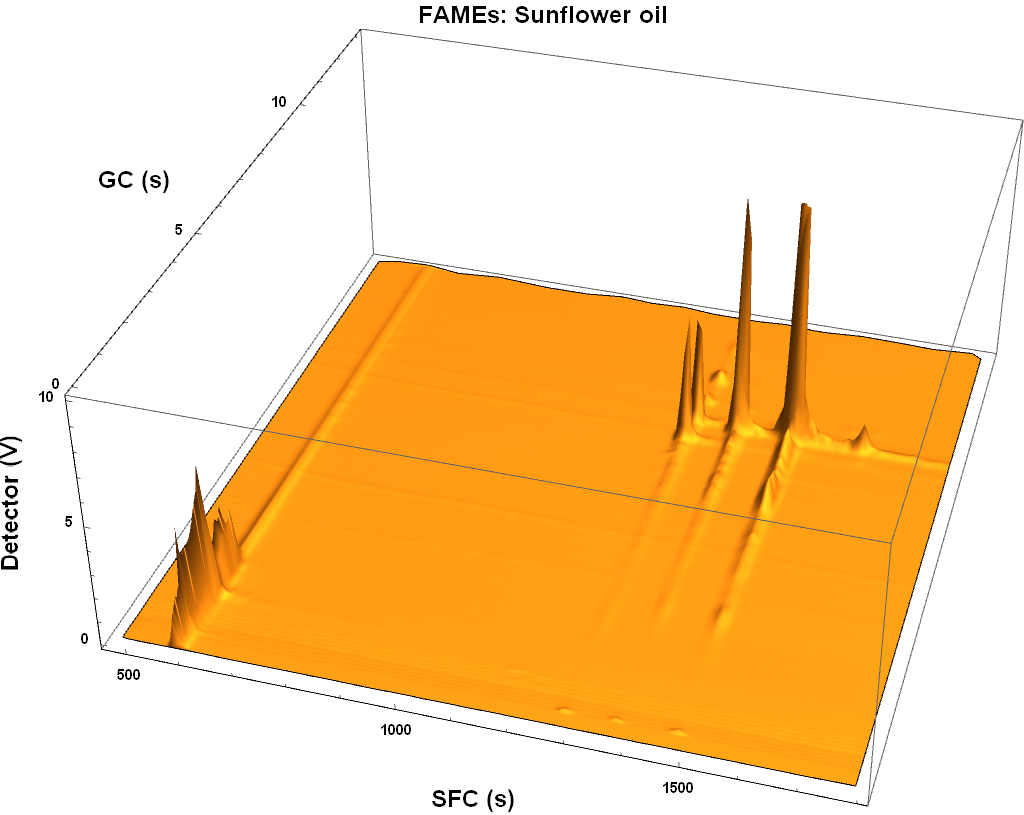
\includegraphics[width=\textwidth]{Figures/Sunflower.png}
\decoRule

\caption[SFC×GC of sunflower oil]{A 2D chromatogram of FAMEs derived from
sunflower oil. It is clear that the oil consists mostly of unsaturated fatty
acids, with a high proportion of linoleic acid (C18:2).}

\label{fig:2DSunflower}
\end{figure}

\subsubsection{Sunflower oil}

Figure \ref{fig:2DSunflower} shows an SFC×GC chromatogram of FAMEs obtained from
sunflower oil. The biggest peak in the chromatogram corresponds to linoleic acid
methyl ester (C18:2). This agrees with the literature, which indicates that the
main, traditional cultivar of sunflower produced in South Africa is of the
high-linoleic type, with a fatty acid profile of \SI{69}{\percent} linoleic
acid, \SI{20}{\percent} oleic acid, and \SI{11}{\percent} saturated fats
\autocite {JFAOWHOCAC2019}.

This sunflower oil chromatogram was compared to a fatty acid profile obtained by
an accredited oil analysis laboratory\footnote{Precision Oil Laboratories,
info@precisionoils.co.za,  +27 15 307 7208, SANAS Testing Laboratory T0802}.
(See Table \ref{tab:SunflowerPrecisionOils}.) The fatty acid profile data was
plotted on a 3D bar chart (See Figure \ref{fig:2DSunflowerBarChart}). The axes
of the bar chart were chosen to plot the fatty acid profile information in a
similar space and scale as the chromatogram (Figure \ref{fig:2DSunflower}). It
can be seen that the bar chart shows the same information as the chromatogram.
The information in the bar chart has been obtained from a 1D chromatogram by
integrating peaks, calculating amounts of FAMEs from peak areas, and then
plotting those amounts in the bar chart, whereas the SFC×GC chromatogram is a
plot of FID response and involves no quantification.

This chromatogram suggests that sunflower oil is a suitable feedstock for
producing biodiesel: the relatively high amount of unsaturated FAs would seem to
imply suitable cold flow properties (see Section \ref{sec:CFPP}). The relatively
high degree of unsaturation does suggest caution regarding oxidative stability
(see Section \ref{sec:Rancimat}).

\begin{figure}
\centering
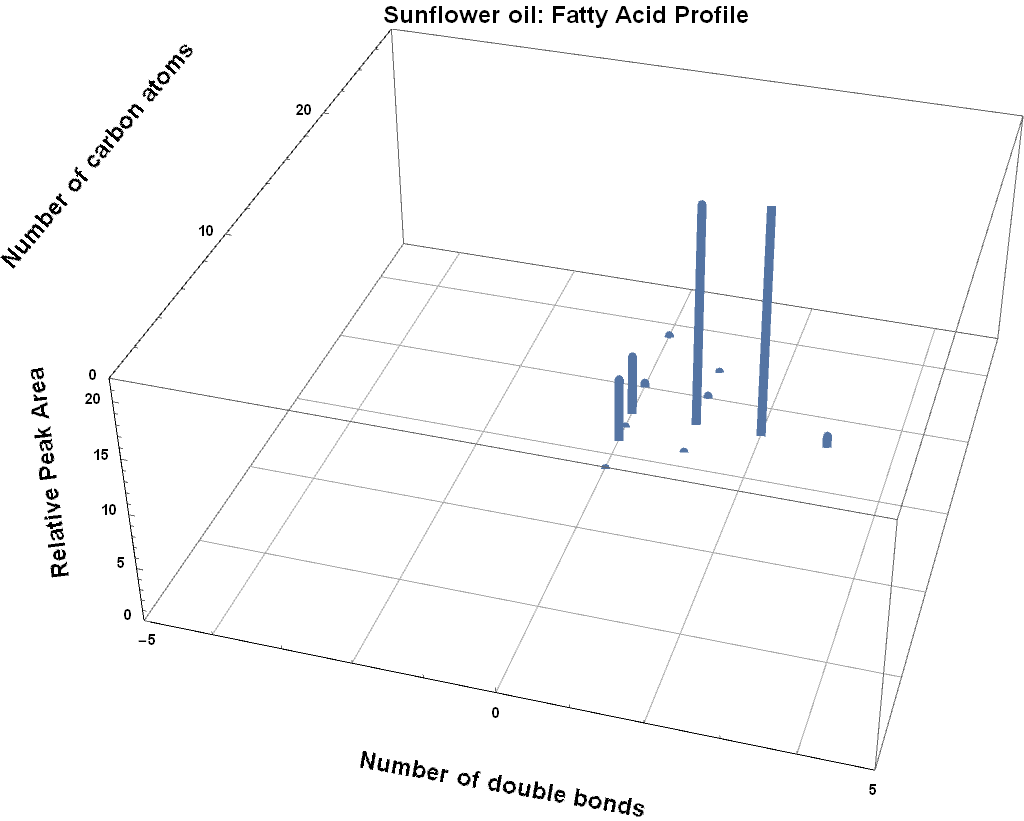
\includegraphics[width=\textwidth]{Figures/BarChart.png}
\decoRule

\caption[3D Bar chart of fatty acid profile]{The fatty acid profile of a
sunflower oil, when plotted on a suitably-scaled bar chart, shows how well the
SFC×GC chromatogram of the same oil (Figure \ref{fig:2DSunflower}) represents
the same data without any processing.}

\label{fig:2DSunflowerBarChart}
\end{figure}

\subsubsection{Coconut oil}

Figure \ref{fig:2DCoconut} shows the SFC×GC chromatogram of FAMES from coconut
oil (\textit{Cocos nucifera L}). It is clear that the dominant FAMEs in coconut
oil are saturated.

The high saturation of coconut oil makes it oxidatively stable (see Section
\refl{sec:Rancimat}), but the high melting point of the saturated FAMEs also
means that it might not meet cold flow requirements (see Section
\ref{sec:CFPP}).

The high oxidative stability of coconut oil makes it resistant to going rancid,
which means it has been used as a natural ingredient for cosmetics since
antiquity \autocite{Berdick1972}.

\begin{figure}
\centering
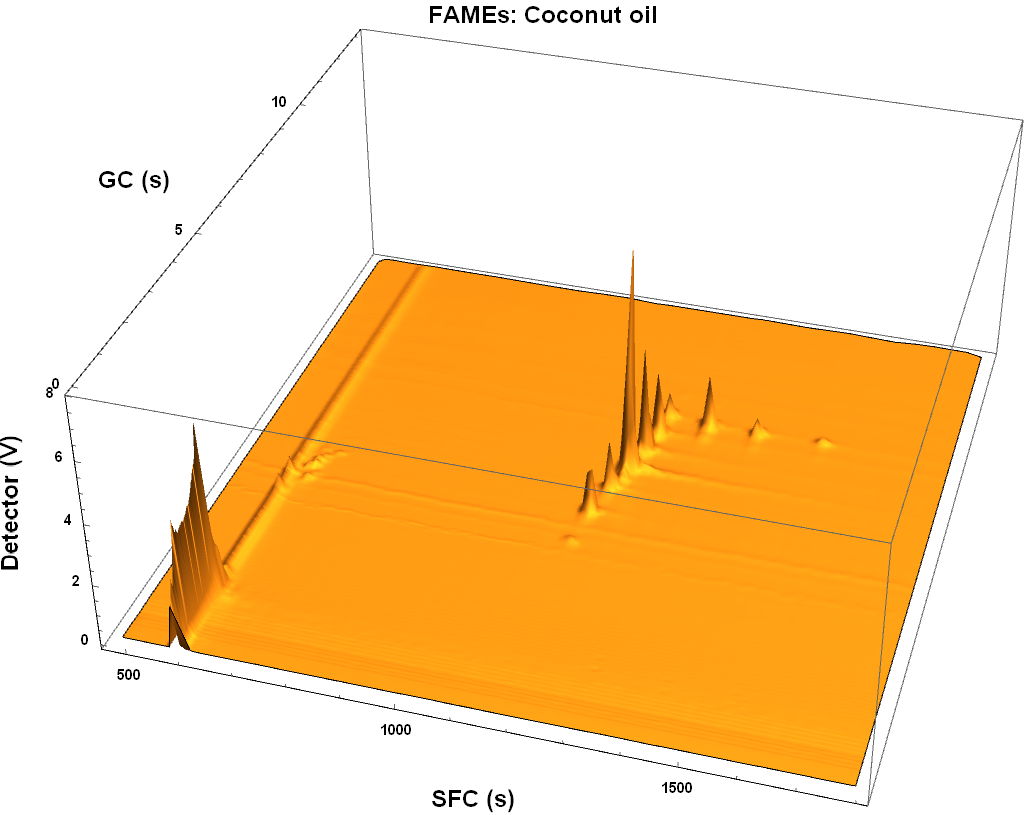
\includegraphics[width=\textwidth]{Figures/Coconut.png}
\decoRule

\caption[SFC×GC of coconut oil]{A 2D chromatogram of FAMEs derived from
coconut oil. It is clear that the oil consists mostly of saturated fatty
acids.}

\label{fig:2DCoconut}
\end{figure}

\subsubsection{Flax seed oil}

Figure \ref{fig:2DFlax} shows an SFC×GC chromatogram of FAMEs obtained from flax
seed oil. This oil is obtained from the seeds of the annual plant \textit{Linum
usitatissimum}, and was sold as an edible oil.

\begin{figure}
\centering
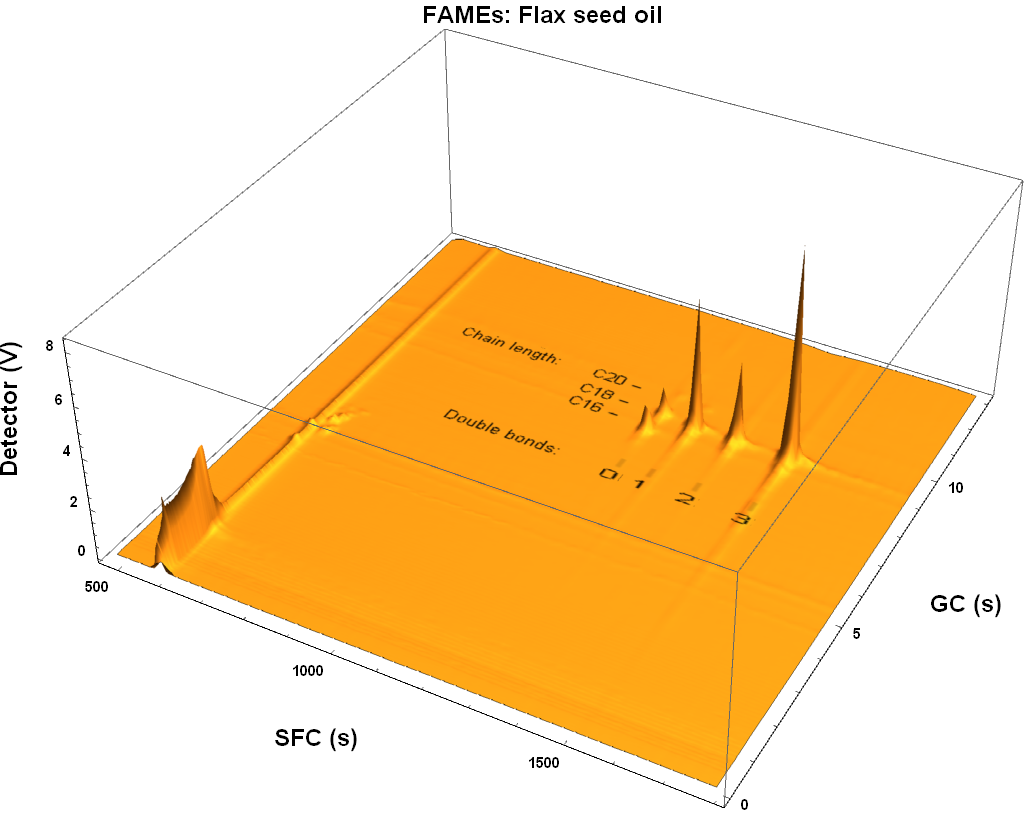
\includegraphics[width=\textwidth]{Figures/Flax.png}
\decoRule

\caption[SFC×GC of flax seed oil]{A 2D chromatogram of FAMEs derived from
flax seed oil. It is clear that the oil consists mostly of highly unsaturated fatty
acids.}

\label{fig:2DFlax}
\end{figure}

The chromatogram shows that the major fatty acid component of flax seed oil is
linolenic acid (C18:3). This will immediately inform a producer that flax seed
oil would not be a suitable feedstock for biodiesel: \std{SANS 1935} limits the
linolenic acid fraction to less than \SI{12}{\percent} (See section
\ref{sec:ChromDetUnsat}).

Flax seed oil only recently became considered a food or a food supplement: the
1911 edition of the Encyclopaedia Britannica only mentions it as a food by
saying ``The oil is to some extent used as food in Russia and in parts of Poland
and Hungary" \autocite{Linseed1911}, and remarks that the oil is edible when it
is cold pressed. This is not surprising, because the oil goes rancid very
quickly, leaving it unpalatable. Historically the more common name for the oil
has been \keyword{linseed oil} and it was mainly used for industrial purposes,
particularly in paint and varnish formulations. As the encyclopedia puts it:
``Commercial linseed oil has a peculiar, rather disagreeable sharp taste and
smell.'' The oil used in artists' oil paints is most commonly refined and
prepared linseed oil. This oil is classed as a \keyword{drying oil}, because a
layer of this oil exposed to air becomes solid, or ``dry". This is the result of
the high degree of unsaturation of the oil, which rapidly causes oxygen-mediated
polymerization. On exposure to air the oil gradually turns more viscous and
eventually solid, making it a suitable base for paint, particularly if the oil
has been pre-treated. In biodiesel such polymerization could cause clogging or
the formation of objectionable sludge.

\subsubsection{Salmon oil}
Figure \ref{fig:2DSalmon} shows an SFC×GC chromatogram of FAMEs obtained from
salmon oil. This oil is obtained from a variety of fish species of the family
\textit{Salmonidae} \autocite{JFAOWHOCAC2017} and was sold as a food
supplement, packaged in gelatine capsules.

\begin{figure}
\centering
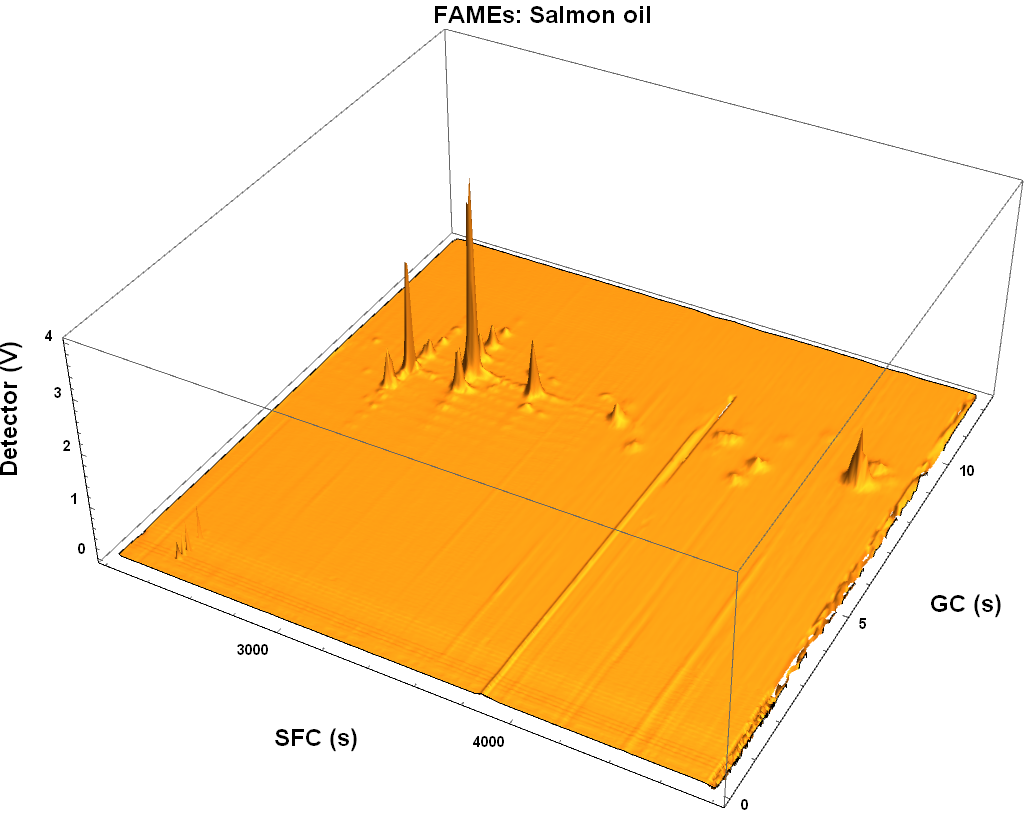
\includegraphics[width=\textwidth]{Figures/Salmon.png}
\decoRule

\caption[SFC×GC of salmon oil]{A 2D chromatogram of FAMEs derived from salmon
oil. It is clear that the oil contains significant quantities of polyunsaturated
fatty acids.}

\label{fig:2DSalmon}
\end{figure}

This chromatogram does not include the \oneD solvent peak. It is much more
complex than the chromatograms of the plant oils shown above. It clearly
shows a degree of unsaturation of up to 5, and there is evidence of a peak that
represents a degree of unsaturation of 6. Unfortunately the instrument started
malfunctioning before this peak could elute completely, and because of a
shortage of time and money the project could not be extended to repair the
instrument, repeat the chromatogram, and confirm the results. 

The fatty acid profile of salmon oil given by the Codex Alimentarius
\autocite{JFAOWHOCAC2017} is shown in Table \ref{tab:SalmonFAO}. Figure
\ref{fig:2DSalmonBarChart} shows the bar-chart representation of the fatty acid
profile. A comparison of the pattern in chromatogram with the bar chart shows
that the chromatogram is consistent with the source of oil being farmed salmon.
The chromatogram also suggests that biodiesel made from salmon oil would not be
compliant with \std{SANS 1935}: the mass fraction of fatty acid methyl esters
with four or more double bonds is more than \SI{1}{\percent}, which is above the
specified limit (see Section \ref{sec:PUFA}).

This complex chromatogram also raises the intriguing possibility of identifying
fatty acid isomers by SFC×GC. This is suggested by the small peaks with a \oneD
retention times slightly different from the main peaks. The identification of
the isomers fall outside the scope of this project, but initial indications are
that, for example, the n-9 isomers of the monounsaturated fatty acids are
slightly less retained than the n-7 isomers. Further studies will be needed to
compare this suspicion to the separation of \textit{cis/trans} isomers of FAMEs
reported by Roger Smith \autocite{Smith2001}.

\begin{figure}
\centering
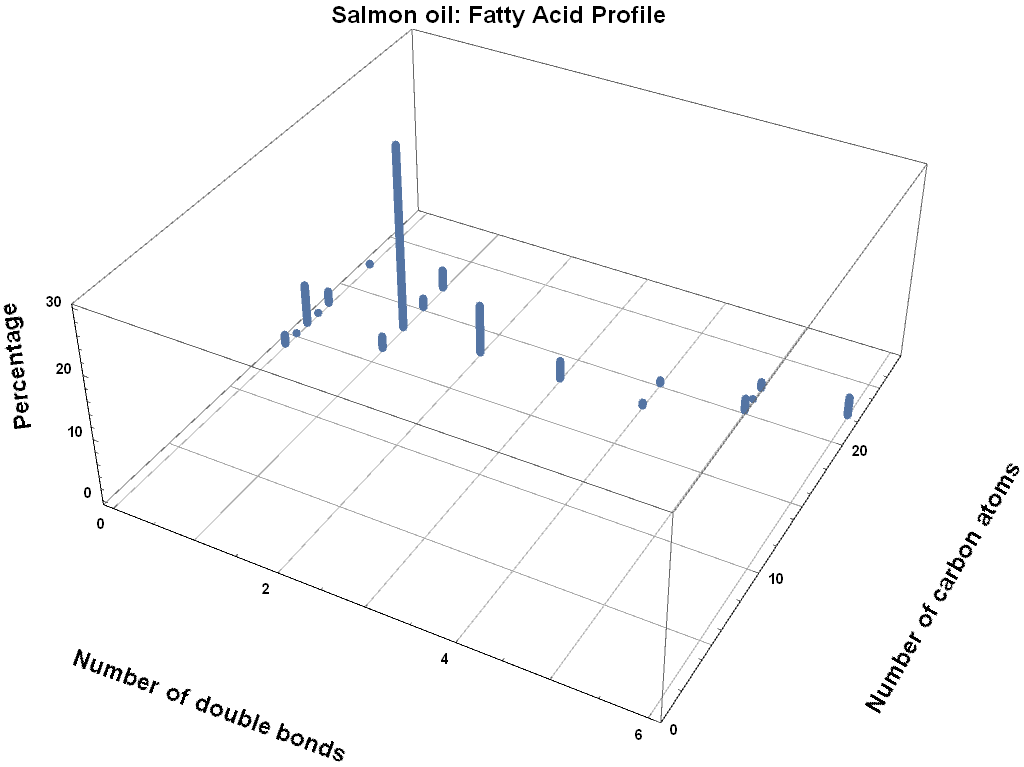
\includegraphics[width=\textwidth]{Figures/SalmonBarChart.png}
\decoRule

\caption[3D Bar chart of salmon oil fatty acid profile]{The fatty acid profile
of salmon oil, when plotted on a suitably-scaled bar chart, shows how well the
SFC×GC chromatogram of the same oil (Figure \ref{fig:2DSalmon}) represents
the same data without any processing.}

\label{fig:2DSalmonBarChart}
\end{figure}

The peak patterns generated in SFC×GC chromatograms of FAME mixtures are
powerful and highly suggestive, but it should be emphasized that patterns are
mere guides and cannot be used to positively identify compounds. Mass
spectrometry can give additional confirmatory information, and injecting
standards is the ultimate method for identifying peaks with compounds. 

\section{Conclusion}

Comprehensively coupled chromatography offers better analytical separations in
three ways: improved peak capacity, improved sensitivity, and more structured
data. The examples presented here do not pretend to prove improved peak
capacity: biodiesel is not normally considered a chromatographically-challenging
complex sample. Neither is improved sensitivity relevant: determining biodiesel
components is not a trace analysis problem for which high sensitivity is
necessary. What these examples do show is that the high orthogonality between
SFC and GC provides data that contains a clear and powerful pattern that greatly
simplifies interpretation. In contrast, Figure \ref{fig:GCxGCFAMEs} shows a
GC×GC chromatogram of a a 37-component FAMEs standard. This separation uses a
polar column in the first dimension, and a non-polar column in the second
dimension \autocite{SepSolveAnalytical2018}. The coloured bands indicates the 2D
retention times of FAMEs with different degrees of unsaturation. The positions
of these bands were determined experimentally using TOF-MS, and are not based on
a separation mechanism. The lower orthogonality of GC×GC, compared to SFC×GC,
means that the position of the bands cannot be predicted, and the shapes of the
bands are likely to change with changing chromatographic conditions.

\begin{figure}[hptb] \centering
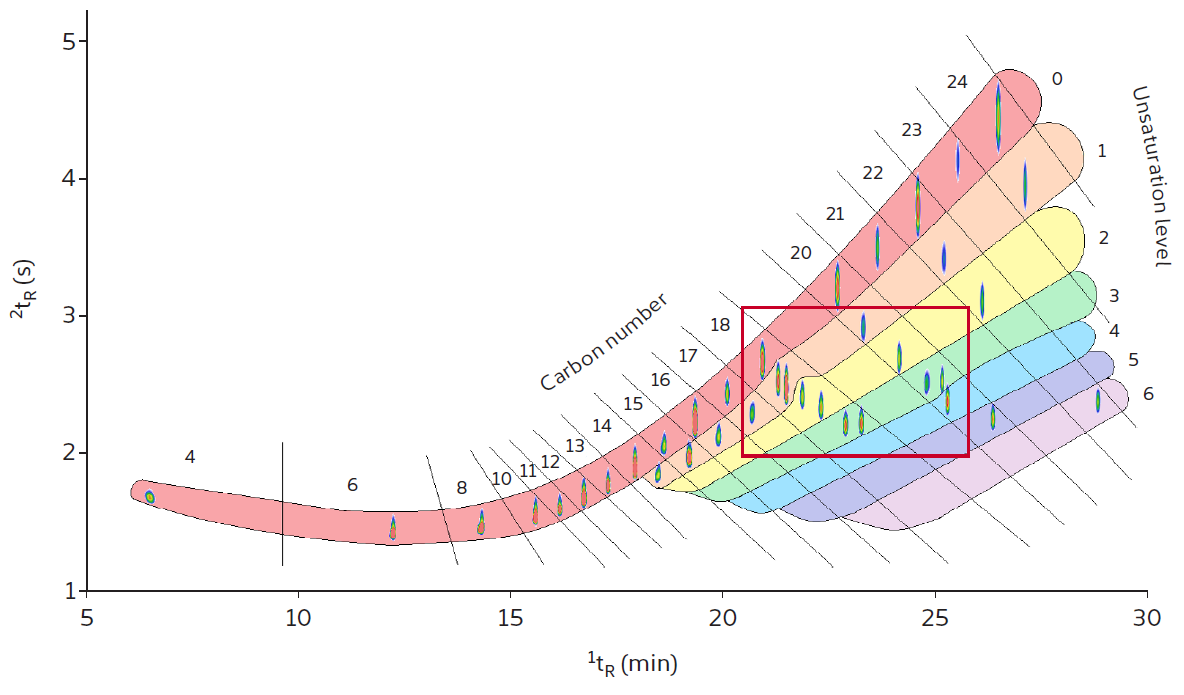
\includegraphics[width=\textwidth]{Figures/GCxGCPattern.png} \decoRule

\caption[GC×GC contour plot]{GC×GC-FID colour plot of a 37-component FAME
standard. The coloured bands indicate successively higher levels of
unsaturation, from 0 (red, no double bonds) to 6 (violet, with 6 double
bonds) \autocite{SepSolveAnalytical2018}.
}

\label{fig:GCxGCFAMEs}
\end{figure}

In the example of FAMEs derived from various oils the pattern shows how the
separation is based on degree of unsaturation in the first dimension and on
volatility in the second dimension. These separations, combined in one 2D
chromatogram, provides intuitive understanding of the chemical composition of
the oils which facilitates prediction about the contribution these oils will
make to the final biodiesel product.

SFC×GC can assist with proving compliance: it provides a chromatographic method
that combines the determination of total FAMEs and unsaturated FAMEs in a single
method. The provided examples also prove that it is possible to design a system
that solves the problems of doing practical, rapidly-repeated fast temperature
programmed GC, ramping temperatures from below ambient to the limits of the
column in hundreds of consecutive, identical runs. This high performance is
possible without resorting to expensive technology.
